\documentclass[finals,table,dvipsnames]{beamer}
\usefonttheme{professionalfonts}

\usepackage[english]{babel}
\usepackage[utf8]{inputenc}
\usepackage[T1]{fontenc}
\usepackage{amsmath}
\usepackage{multicol}
\usepackage{graphicx}
\usepackage{hyperref}
\usepackage{float}
\usepackage{url}
\usepackage{wasysym}
\usepackage{xspace}
\usepackage{times}
\usepackage{booktabs}
\usepackage{xcolor}
\usepackage{marvosym}
\usepackage{tikz}
\usepackage{listings}
\usepackage{fancybox}
\usepackage{shadow}


\usetikzlibrary{arrows,shapes,backgrounds}
\tikzstyle{every picture}+=[remember picture]
\tikzstyle{na} = [baseline=-.5ex]

\DeclareGraphicsExtensions{.eps,.pdf,.JPG,.jpg,.jpeg,.png,.PNG}
\graphicspath{
{./figures/}
}
\definecolor{sdnblue}{HTML}{005baa}
\definecolor{sdngrey}{HTML}{646464}

\setbeamertemplate{navigation symbols}{}
\setbeamercolor{title}{fg=sdnblue}
\setbeamertemplate{footline}[frame number]
%\setbeamercolor{background canvas}{bg=black!95}
%\setbeamercolor{normal text}{bg=black,fg=white}
\setbeamercolor{frametitle}{fg=sdnblue}
%\setbeamercolor{section in sidebar}{fg=blue!70}
%\setbeamercolor{sidebar}{fg=black}
%\setbeamercolor{structure}{bg=black,fg=black!5}
%\setbeamercolor{item projected}{fg=black,bg=white}


\setbeamertemplate{items}[square] 
\setbeamertemplate{caption}[numbered]
\setbeamerfont{caption}{size=\scriptsize,family=\it}
\usefonttheme{professionalfonts} % using non standard fonts for beamer
\usefonttheme{serif} % default family is serif

%--------------------------------
\hypersetup{bookmarksopen=true,
bookmarksnumbered=true,  
pdffitwindow=true, 
pdfstartview=Fit,
%pdfpagemode=FullScreen,
pdffitwindow=true,
pdftoolbar=true,
pdfmenubar=true,
pdfwindowui=true,
pdfauthor={Alexander Barth{,} Aida Alvera-Azc\'{a}rate{,} Mohamed~Ouberdous{,} Charles~Troupin{,} Sylvain~Watelet \& Jean-Marie~Beckers},
pdfsubject={DIVA Lecce 2016},
pdftitle={DIVA Lecce 2016},
bookmarksopenlevel=0,
colorlinks=true,
linkcolor=blue,anchorcolor=black,%
citecolor=blue,filecolor=black,%
menucolor=black,urlcolor=blue,%
pdfpageduration=1,%
pdffitwindow=true
}

\logo{\vspace{-5mm}
\includegraphics[height=0.5cm]{gherlogo_transparent}~
\includegraphics[height=0.5cm]{Logo_SeaDataNet_fond_transparent}\hspace{7mm}}

\author[Alexander Barth, Aida Alvera-Azc\'{a}rate, Mohamed~Ouberdous, Charles~Troupin, Sylvain~Watelet \& Jean-Marie~Beckers]{Alexander Barth, Aida Alvera-Azc\'{a}rate, Mohamed~Ouberdous,\\
 Charles~Troupin, Sylvain~Watelet \& Jean-Marie~Beckers}
  
\title[]{\diva Lecce 2016}
\date{Lecce (Italy), 11--14 April 2016}


%--------------------------------

\definecolor{colorcite}{rgb}{0,.46,.46}
\newcommand{\diva}{\textsf{Diva}\xspace}
\newcommand{\mat}{\mathbf}
\newcommand{\important}[1]{\textcolor{sdnblue}{#1}}
\newcommand{\method}[1]{\textcolor{gray}{#1}}
\newcommand{\tool}[1]{\textcolor{sdngrey}{\texttt{#1}}}
\newcommand{\nablab}{\boldsymbol{\nabla}}
\newcommand{\ddiff}{\mbox{d}}
\newcommand{\cita}[1]{\textcolor{colorcite}{#1}}
\newcommand{\fleche}{$\rightarrow$\,}
\newcommand{\snr}{\lambda}
\newcommand{\noise}{\epsilon}

\newcommand{\directory}[1]{\texttt{\color{ForestGreen}{#1}}}
\newcommand{\file}[1]{\texttt{\color{MidnightBlue}{#1}}}
\newcommand{\command}[1]{\texttt{\color{RedOrange}{#1}}}
\newcommand{\resfile}[1]{\texttt{\color{MidnightBlue}{#1}}}

\newcommand{\statmean}[1]{\left\langle #1 \right\rangle}
\newcommand{\true}[1]{{#1}^t}
\newcommand{\analyzed}[1]{{#1}^a}
\newcommand{\observation}{ \mbox{\boldmath   $ \protect\mathrm{y} $} }
\newcommand{\forecasted}[1]{{#1}^f}
\newcommand{\kalmangain}{\matr{K}}
\newcommand{\Hobs}{\matr{H}}
\newcommand{\errorv}{\vect{\epsilon}}
\newcommand{\errorobs}{\vect{\epsilon}^o}
\newcommand{\Perr}{\matr{P}}
\newcommand{\Rerr}{\matr{R}}

\newcommand{\matr}[1] { \mbox{\boldmath   $ \protect\mathsf{#1} $} }
\newcommand{\trcon}[1]{{#1}^\star}
\newcommand{\adj}[1]{\trcon{#1}}
\newcommand{\elem}[2]{\left( #1 \right)_{#2}}
\newcommand{\trace}{\operatorname{trace}}
\newcommand{\sing}{\rho}

\newcommand{\myshadowbox}[1]{\shabox{\parbox{10cm}{#1}}}
\newcommand{\inv}[1]{{#1}^{ \mbox{\small{-}}  1}}

\lstdefinestyle{Bash}
{language=bash,
keywordstyle=\color{blue},
basicstyle=\ttfamily,
morekeywords={ctroupin@gher13},
alsoletter={:~$},
commentstyle=\color{dkgreen},
morekeywords=[2]{ctroupin@gher13:},
keywordstyle=[2]{\color{red}},
literate={\$}{{\textcolor{red}{\$}}}1 
         {:}{{\textcolor{red}{:}}}1
         {~}{{\textcolor{red}{\textasciitilde}}}1,
}
\lstset{
    breaklines     = true,
    frame          = single,
    rulecolor=     \color{gray},
}

%$

%-------------------------------------------------------------------------
\newcommand{\maketitlepage}{{
\usebackgroundtemplate{\hspace{-1cm}\tikz\node[opacity=0.2]{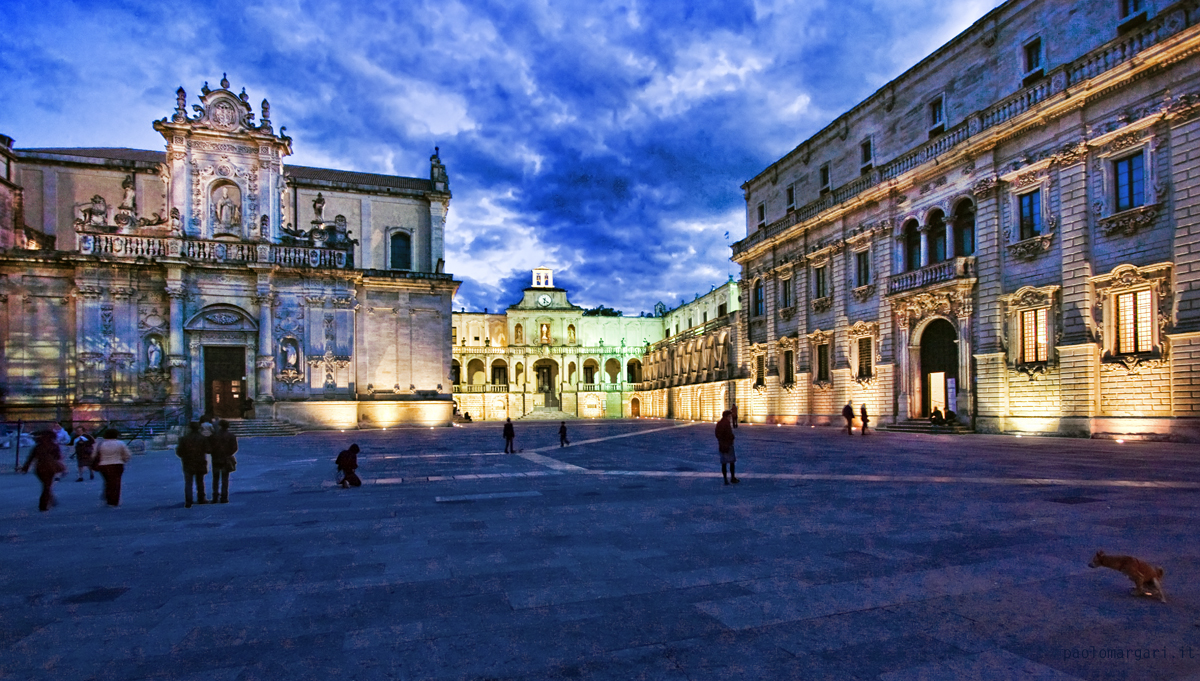
\includegraphics[height=1.05\paperheight]{Lecce1.jpg}};}
\begin{frame}
\centering
\footnotesize
\maketitle
\vspace{-.25cm}
\tiny{\textbf{Acknowledgements:} SeaDataNet, EMODnet Chemistry, \\
EMODnet Biology, STARESO}
\vspace{.125cm}

\begin{figure}
\centering

\includegraphics[width=.1\paperwidth]{gherlogo_transparent.PNG}\hspace*{.5cm}
\includegraphics[width=.1\paperwidth]{logo_ulg}\hspace*{.5cm}
\includegraphics[width=.1\paperwidth]{Logo_SeaDataNet_fond_transparent}\hspace*{.5cm}
\includegraphics[width=.07\paperwidth]{logo_emodnet}\hspace*{.5cm}
\includegraphics[width=.09\paperwidth]{Logo_Stareso}
\end{figure}

\end{frame}
}}
%-------------------------------------------------------------------------

\parindent 0cm

\subtitle{General information}

\begin{document}

\maketitlepage % defined in GHERheader2013.tex

%--------------------------------------------------------------------------------------------------------


\begin{frame}
\frametitle{Welcome to Lecce}
\footnotesize

\onslide*<1>{
\begin{figure}
\centering
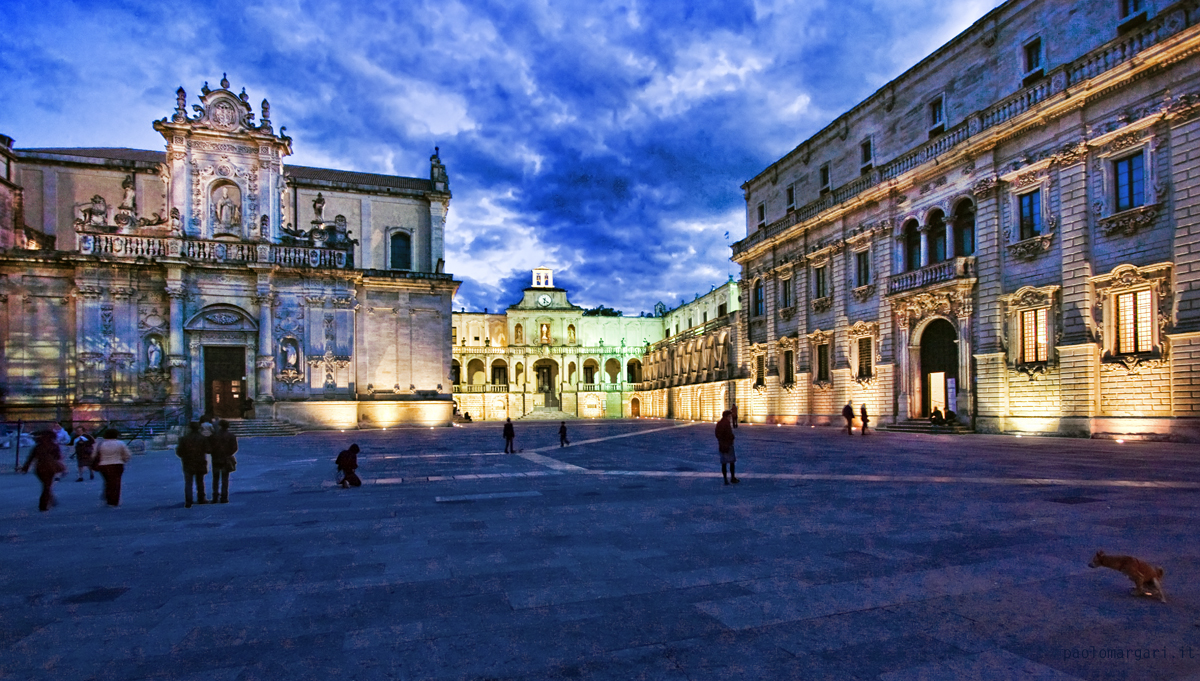
\includegraphics[width=.99\textwidth]{Lecce1}
\end{figure}
}

%\onslide*<2>{

%\begin{columns}[totalwidth=\textwidth]

%\column{.5\textwidth}
%\begin{figure}
%\centering
%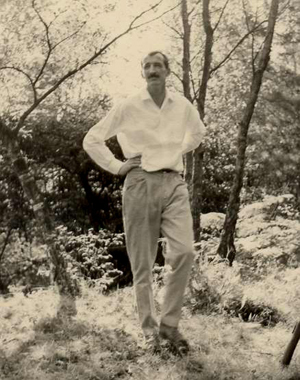
\includegraphics[width=.8\textwidth]{stebelle}
%\end{figure}

%\column{.5\textwidth}

%\begin{description}
%\item[Origin:] recteur Marcel Dubuisson (1972)
%\item[Architect:] Claude Strebelle (1917-2010) 
%\item[Management:] STARESO S.A. (1989)
%\end{description}
%\url{http://www.stareso.ulg.ac.be}

%\end{columns}
%}

%Cap de la Revellata 
% %pollution inexistante
%Architecte Claude Strebelle: pierres de granit (invisible depuis le large)






\end{frame}

%------------------------------------------------------------------------------------

\begin{frame}[t]
\frametitle{Previous workshops}

\begin{columns}[totalwidth=1.1\textwidth,c]

\column{.55\textwidth}
\begin{description}
\footnotesize
\item[November 13-15, 2006:] Li\`{e}ge
\item[November 4-6, 2007:] STARESO
\item[October 15-17, 2008:] STARES
\item[October 23-26, 2009:] STARESO
\item[November 3-6, 2010:] STARESO
\item[October 8-12, 2012:] Roumaillac
\item[November 4-8, 2013:] STARESO
\item[November 3-7, 2014:] STARESO
\end{description}

\begin{figure}
\centering
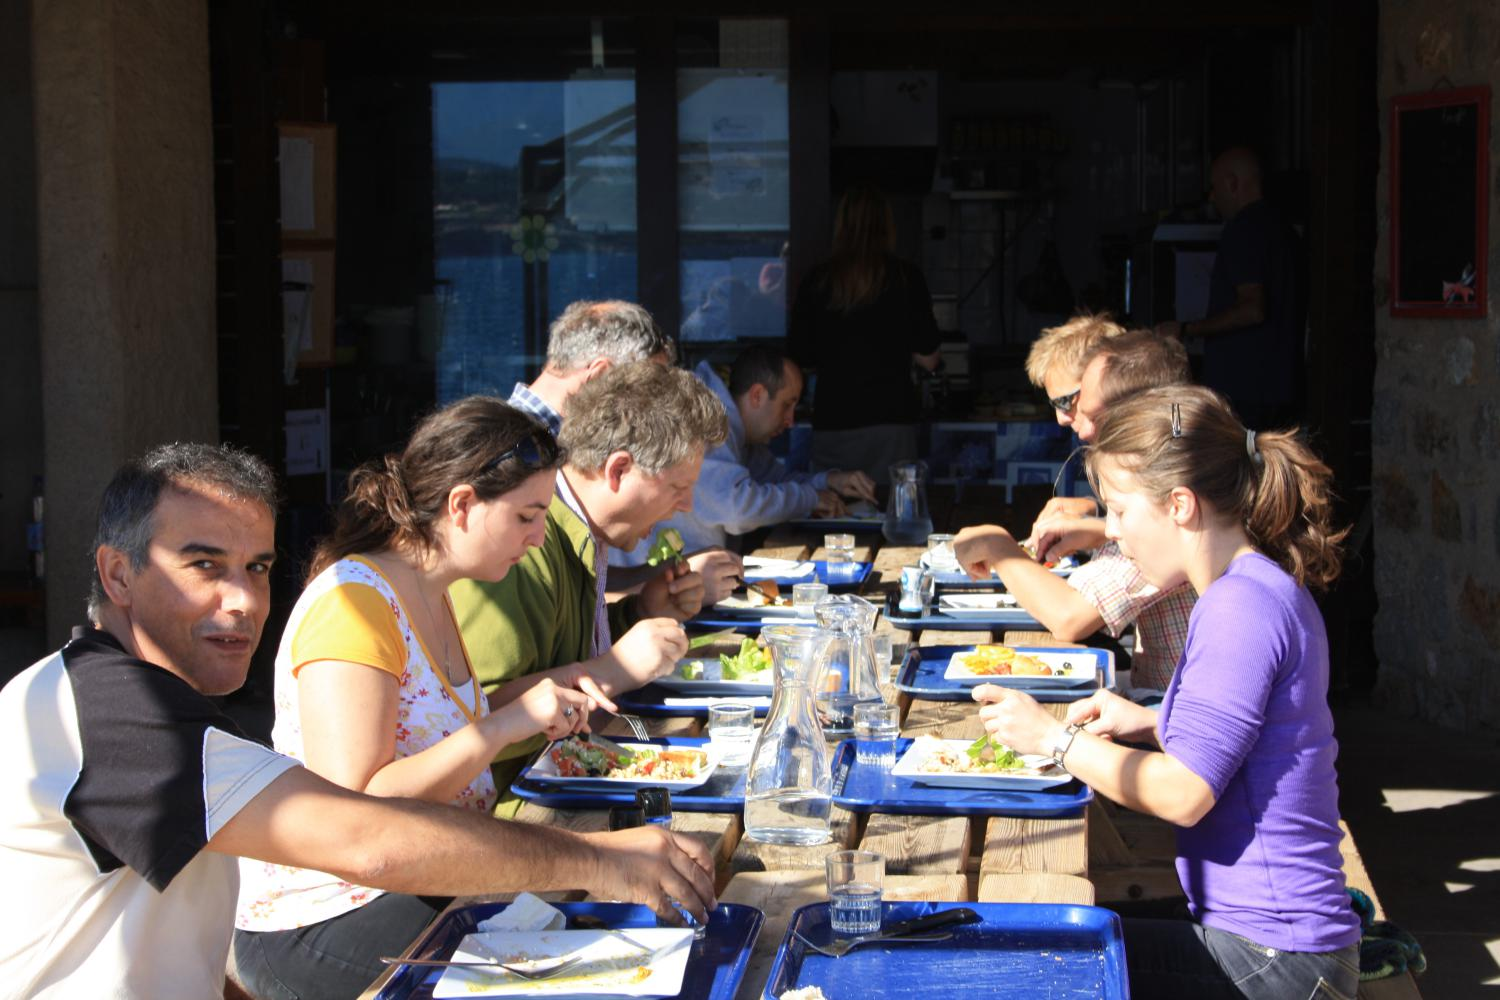
\includegraphics[width=5cm]{IMG_6061.JPG}
\end{figure}

\column{.55\textwidth}
\begin{figure}
\centering
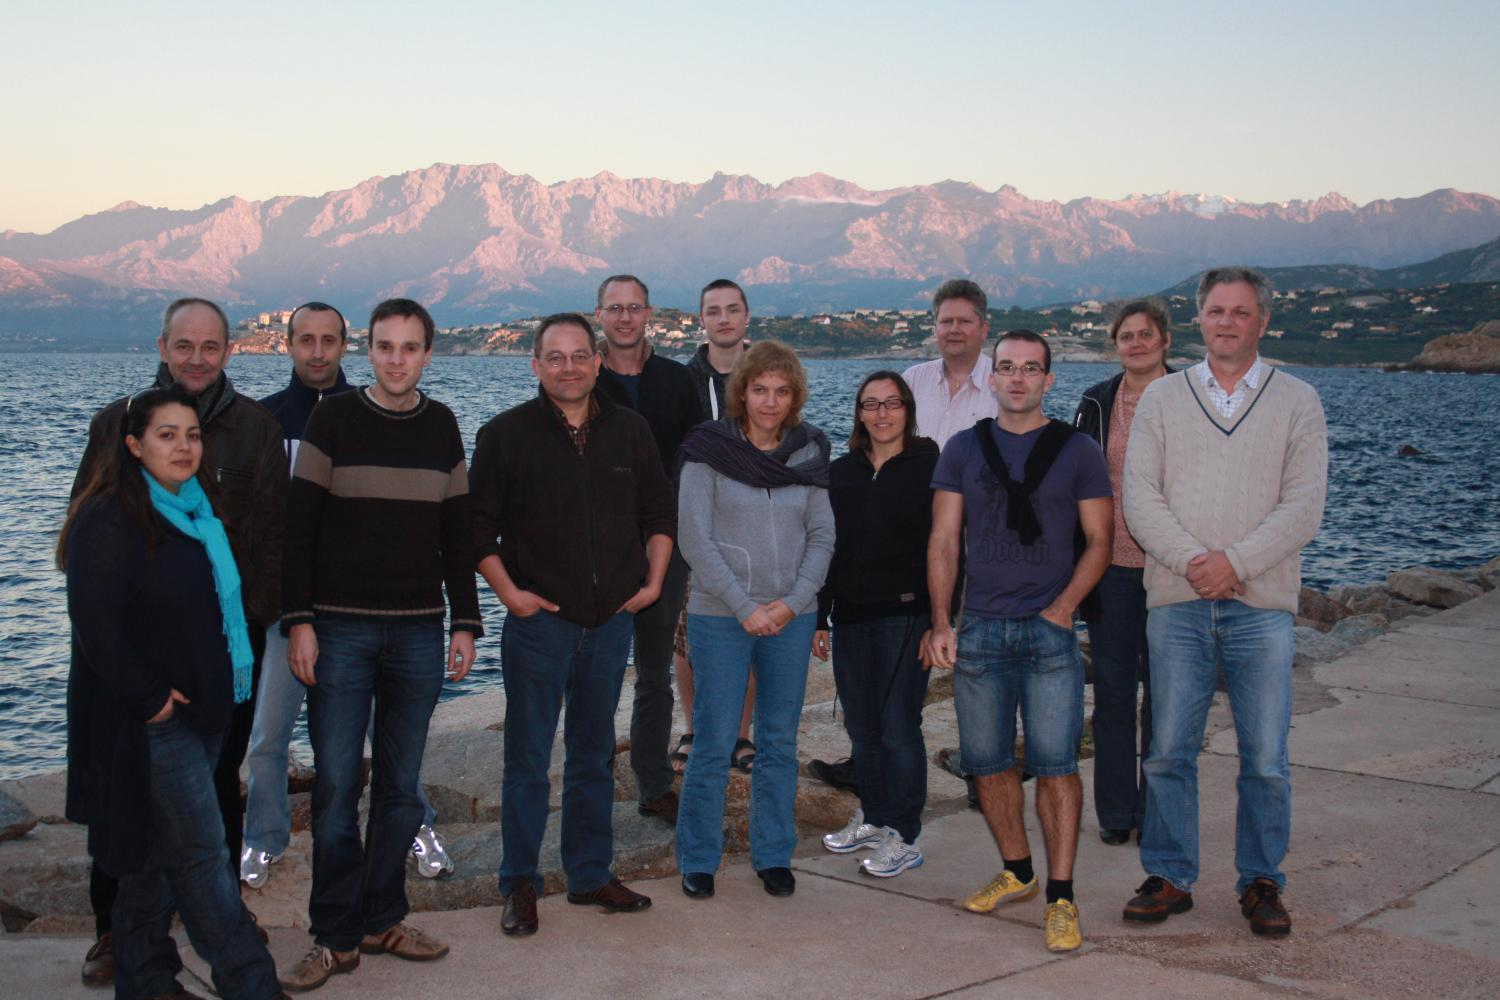
\includegraphics[width=5cm]{IMG_7268.JPG}
\vspace*{2.5mm}
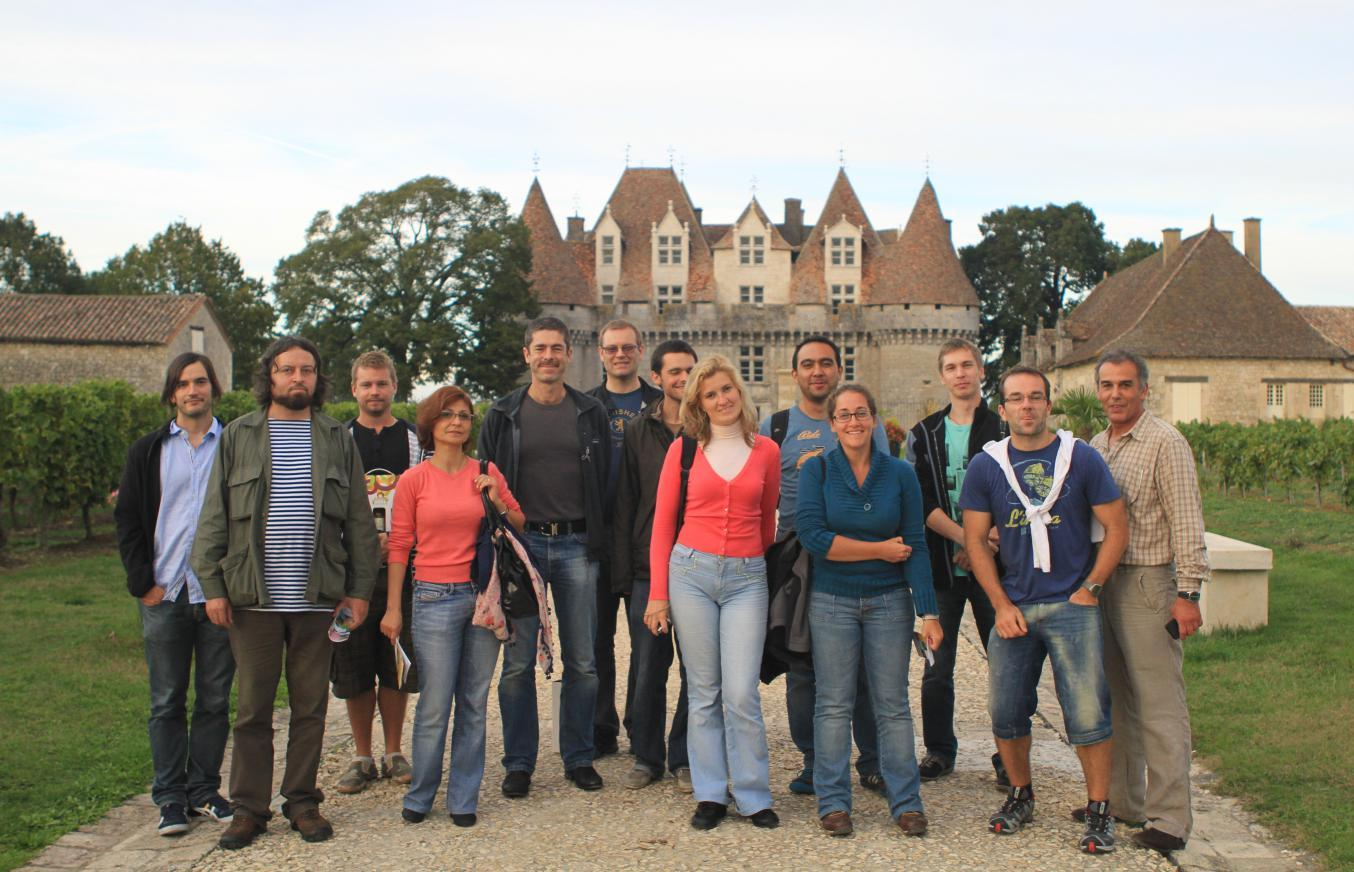
\includegraphics[width=5cm]{Workshop2012}
\end{figure}
\end{columns}

\end{frame}


%--------------------------------------------------------------------------------------------
\begin{frame}[t]
\frametitle{General organization}
\footnotesize

\begin{columns}[totalwidth=\textwidth,c]

\column{.55\textwidth}

\begin{description}

\item[Program:] user-driven 
\item[Morning lectures:] from 9:00 to 18:00
\item[Lunch:] 13:00 to 14:30
\item[Afternoon exercises:] from 14:30 to 18:00

%Listen to the bell!
%\item[Drinks:] ? %write your name/consumptions on the blackboard
%\item[]
%\item[Internet:] ? %wireless in the station,\\
%not in the lighthouse
\end{description}

\column{.45\textwidth}
{
\begin{figure}
\centering
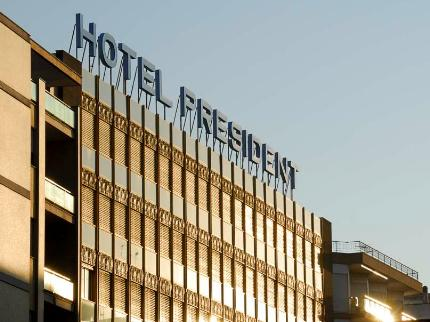
\includegraphics[width=.7\textwidth]{president-lecce}
\end{figure}
}
\end{columns}
\end{frame}


%------------------------------------------------------------------------------------
\begin{frame}[t]
\frametitle{Program}
\footnotesize

\onslide*<1-4>{\vspace{2cm}}

\onslide*<1>{
\important{Monday 11}
\begin{itemize}
\scriptsize
\item[\CheckedBox] Presentation of \diva software (formulation, advantages, implementation)
\item[\CheckedBox] Tests with a common data set in 2D (influence of analysis parameters and error field calculation)
\item[\CheckedBox] Extraction of topography and creation of contours from topography
\item[\CheckedBox] Presentation of \diva-on-web and OceanBrowser
\item[\CheckedBox] Registration to the \diva user group \url{https://groups.google.com/forum/\#!forum/diva_users}
\end{itemize}
}
\onslide*<2>{
\important{Tuesday 12}
\begin{itemize}
\scriptsize
\item[\CheckedBox] Presentation of GODIVA (Diva with loops on time and depth levels)
\item[\CheckedBox] Test case with a common data set: role of the parameters in the driver file
\item[\CheckedBox] Extraction of data from ODV spreadsheets
\item[\CheckedBox] Application with provided data set
\end{itemize}
}
\onslide*<3>{
\important{Wednesday 13}
\begin{itemize}
\scriptsize
\item[\CheckedBox] Presentation: recent developments and future improvements of Diva
\item[\CheckedBox] Methods to derive error fields
\item[\CheckedBox] Application with provided data set (continued)
\item[\CheckedBox] Advanced analysis (for expert users): advection, data transformation, correlated observational errors
\end{itemize}
}
\onslide*<4>{
\important{Thursday 14}
\begin{itemize}
\scriptsize
\item[\CheckedBox] Extension of DIVA to higher dimensions
\item[\CheckedBox] Analytical solutions and well-posed character of the problem
\item[\CheckedBox] Advection constraint with time dimension
\item[\CheckedBox] Multivariate extension
\item[\CheckedBox] Presentation of the participants results (?)
\item[\CheckedBox] User specific questions + feedback.
\end{itemize}
}
\onslide*<5>{
\begin{columns}[totalwidth=\textwidth]
\column{.525\textwidth}

\important{Monday 11}
\begin{itemize}
\scriptsize
\item[\CheckedBox] Presentation of \diva software (formulation, advantages, implementation)
\item[\CheckedBox] Tests with a common data set in 2D (influence of analysis parameters and error field calculation)
\item[\CheckedBox] Extraction of topography and creation of contours from topography
\item[\CheckedBox] Presentation of \diva-on-web and OceanBrowser
\item[\CheckedBox] Registration to the \diva user group \url{https://groups.google.com/forum/\#!forum/diva_users}
\end{itemize}

\important{Tuesday 12}
\begin{itemize}
\scriptsize
\item[\CheckedBox] Presentation of GODIVA (Diva with loops on time and depth levels)
\item[\CheckedBox] Test case with a common data set: role of the parameters in the driver file
\item[\CheckedBox] Extraction of data from ODV spreadsheets
\item[\CheckedBox] Application with provided data set
\end{itemize}

\column{.525\textwidth}

\important{Wednesday 13}
\begin{itemize}
\scriptsize
\item[\CheckedBox] Presentation: recent developments and future improvements of Diva
\item[\CheckedBox] Methods to derive error fields
\item[\CheckedBox] Application with provided data set (continued)
\item[\CheckedBox] Advanced analysis (for expert users): advection, data transformation, correlated observational errors
\end{itemize}

\important{Thursday 14}
\begin{itemize}
\scriptsize
\item[\CheckedBox] Extension of DIVA to higher dimensions
\item[\CheckedBox] Analytical solutions and well-posed character of the problem
\item[\CheckedBox] Advection constraint with time dimension
\item[\CheckedBox] Multivariate extension
\item[\CheckedBox] Presentation of the participants results (?)
\item[\CheckedBox] User specific questions + feedback.
\end{itemize}

\end{columns}
}
\end{frame}

%--------------------------------------------------------------------------------------------------------

% \begin{frame}
% \frametitle{Who's attending the workshop?}

% \begin{figure}
% \centering
% \onslide*<1>{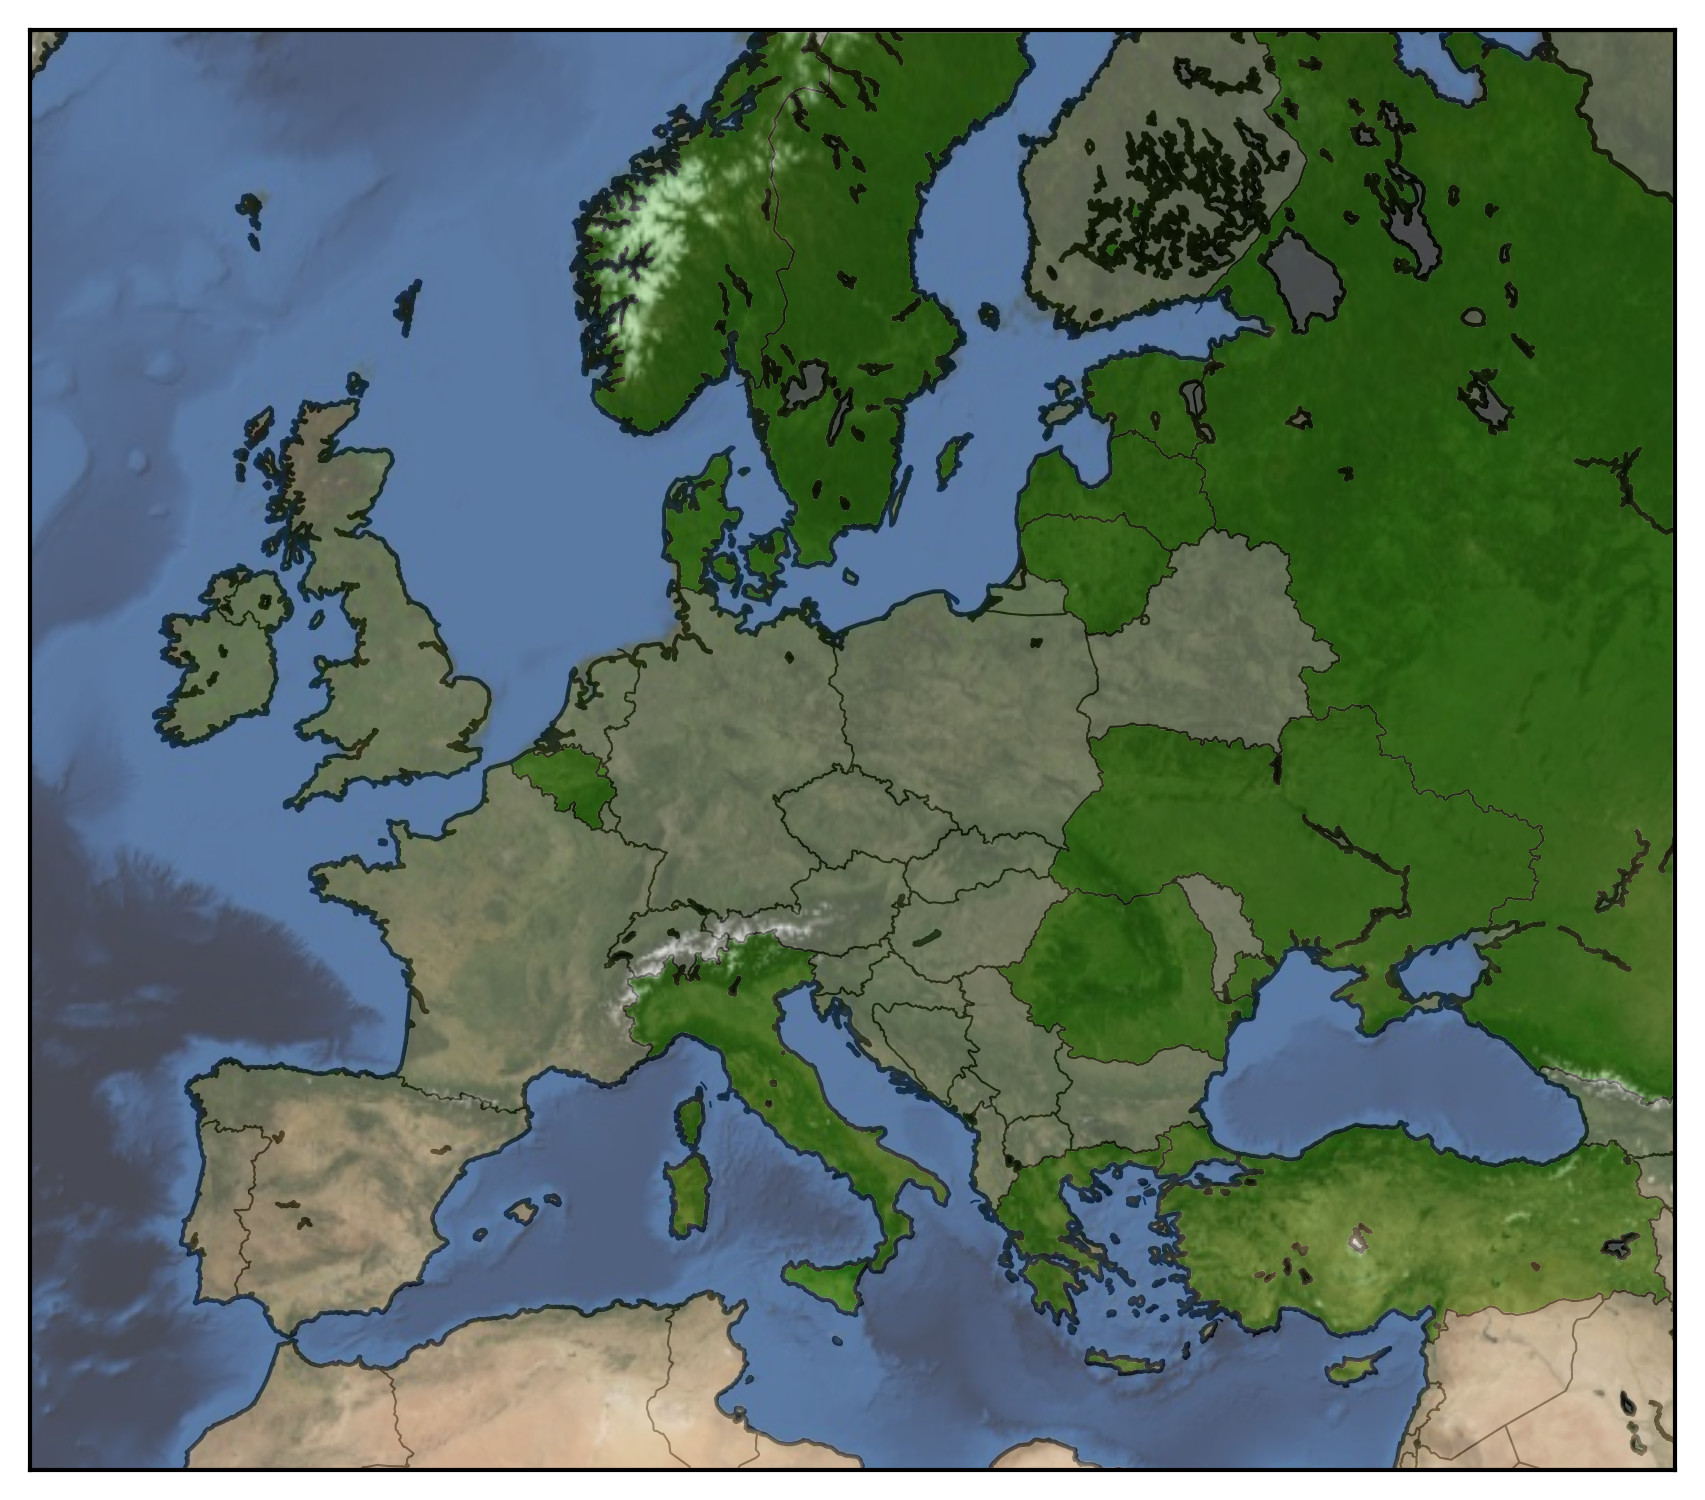
\includegraphics[width=.8\textwidth]{participant_map2.jpg}}
% \onslide*<2>{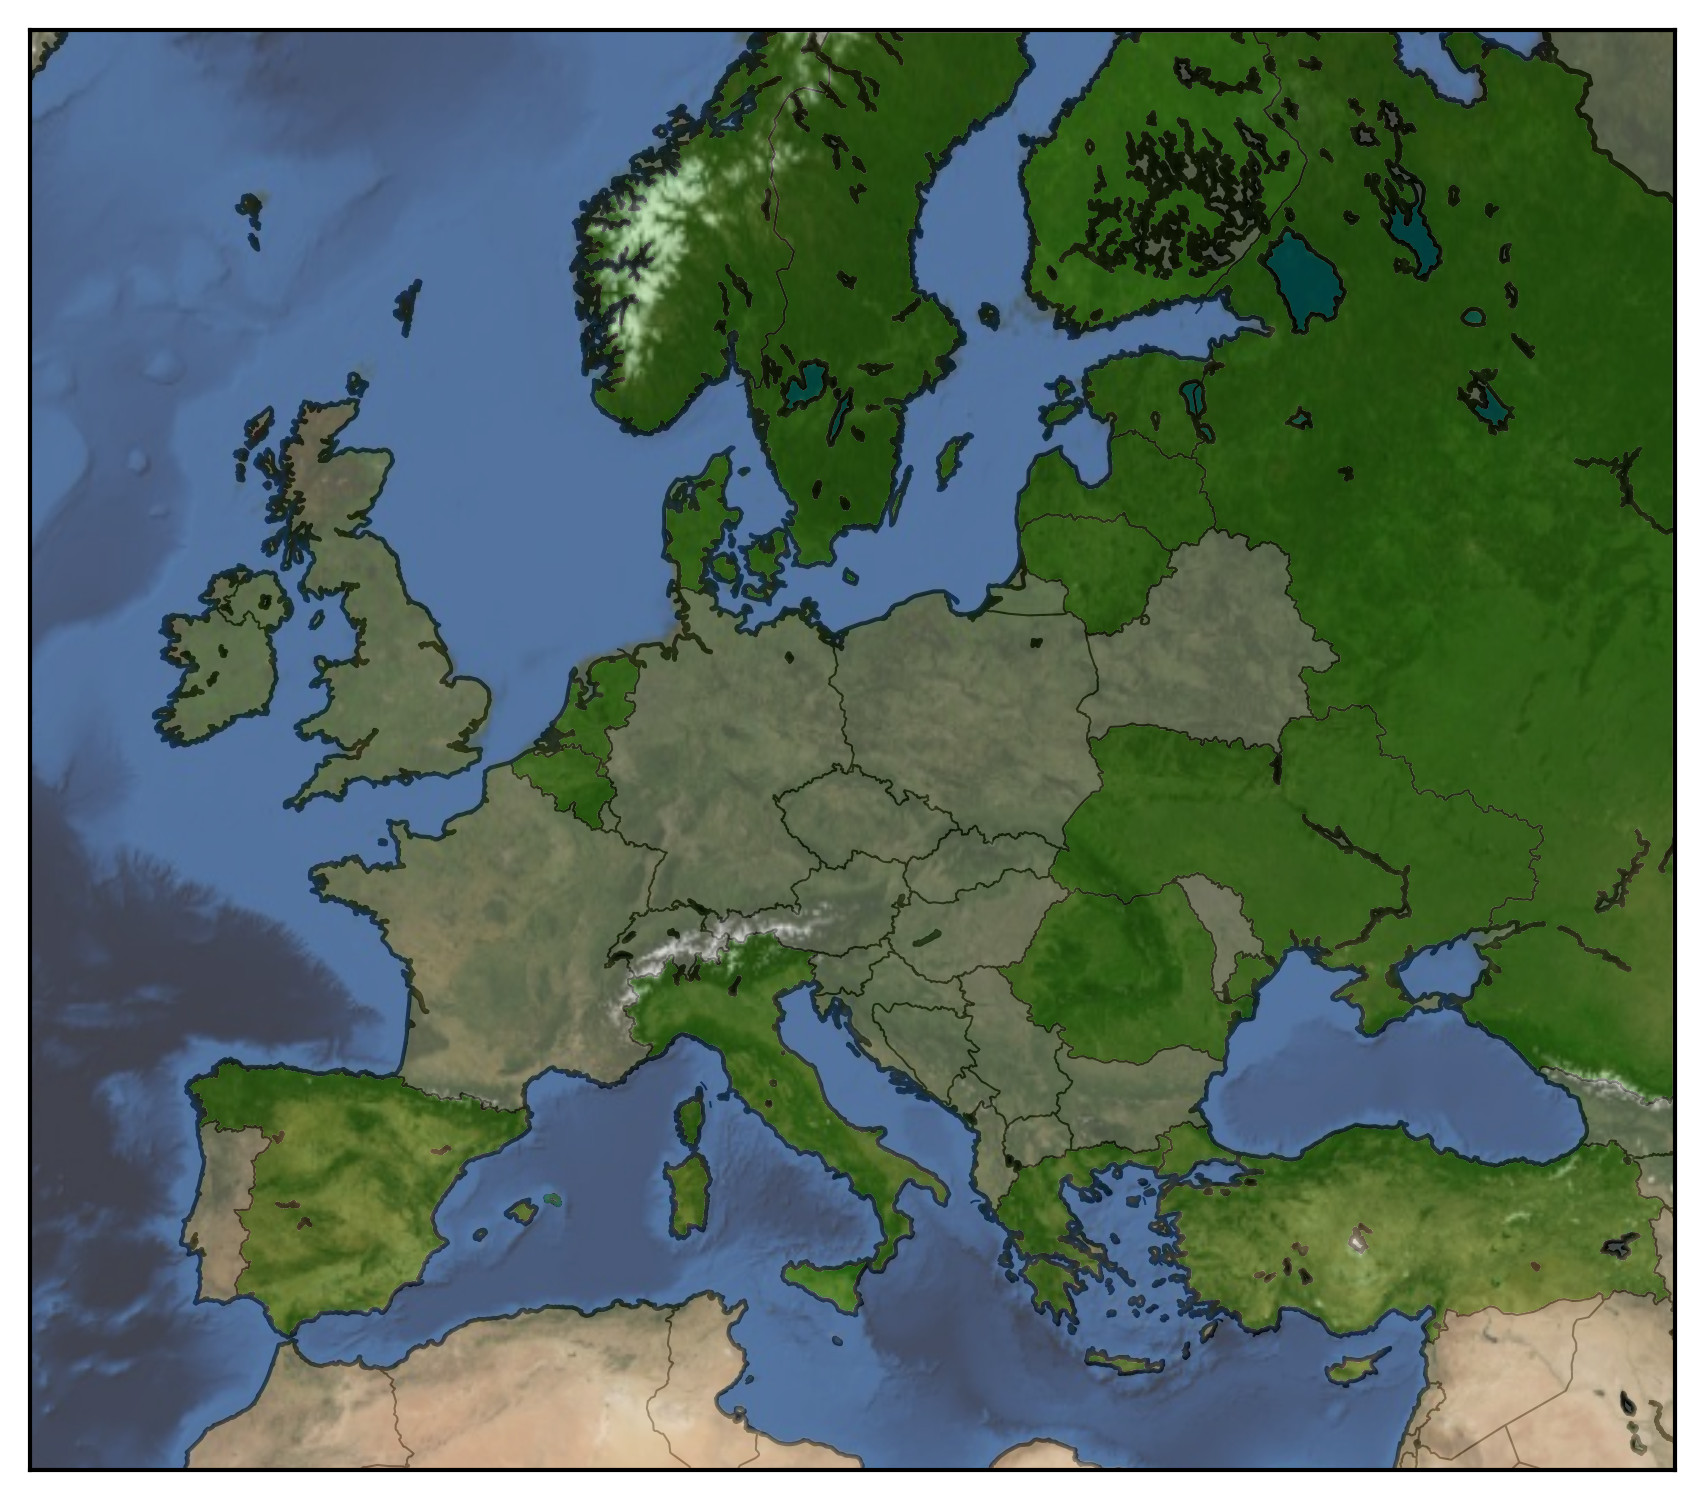
\includegraphics[width=.8\textwidth]{participant_map4.jpg}}
% \end{figure}


% \end{frame}

%--------------------------------------------------------------------------------------------------------

\begin{frame}
\frametitle{The GHER-\diva team}

\begin{tabular}{lrclr}
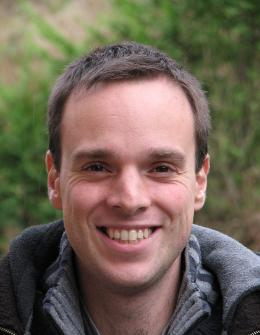
\includegraphics[width=.15\textwidth]{alex.jpg} & Alexander &&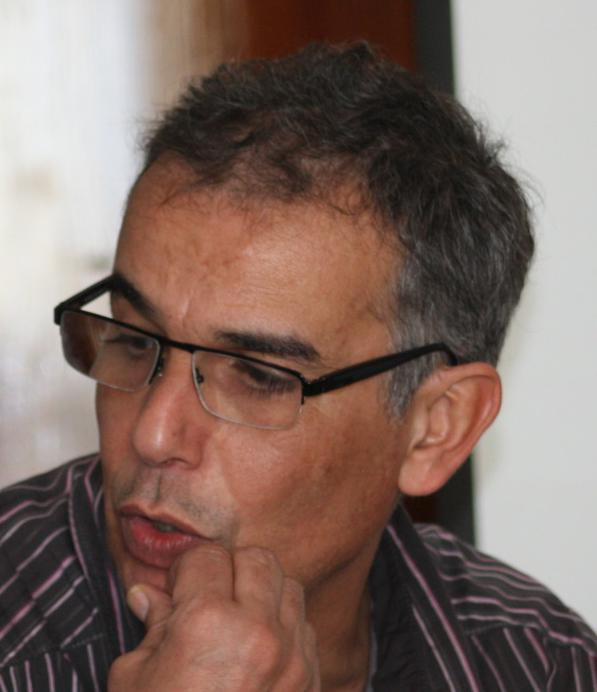
\includegraphics[width=.15\textwidth]{mohamed2.jpg} & Mohamed \\
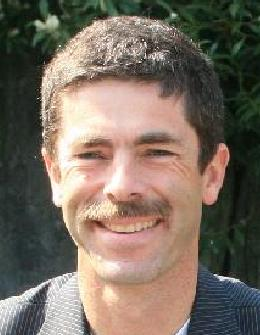
\includegraphics[width=.15\textwidth]{jmb.jpg} & Jean-Marie && 
\includegraphics[width=.15\textwidth]{sylvain3.jpg} & Sylvain \\
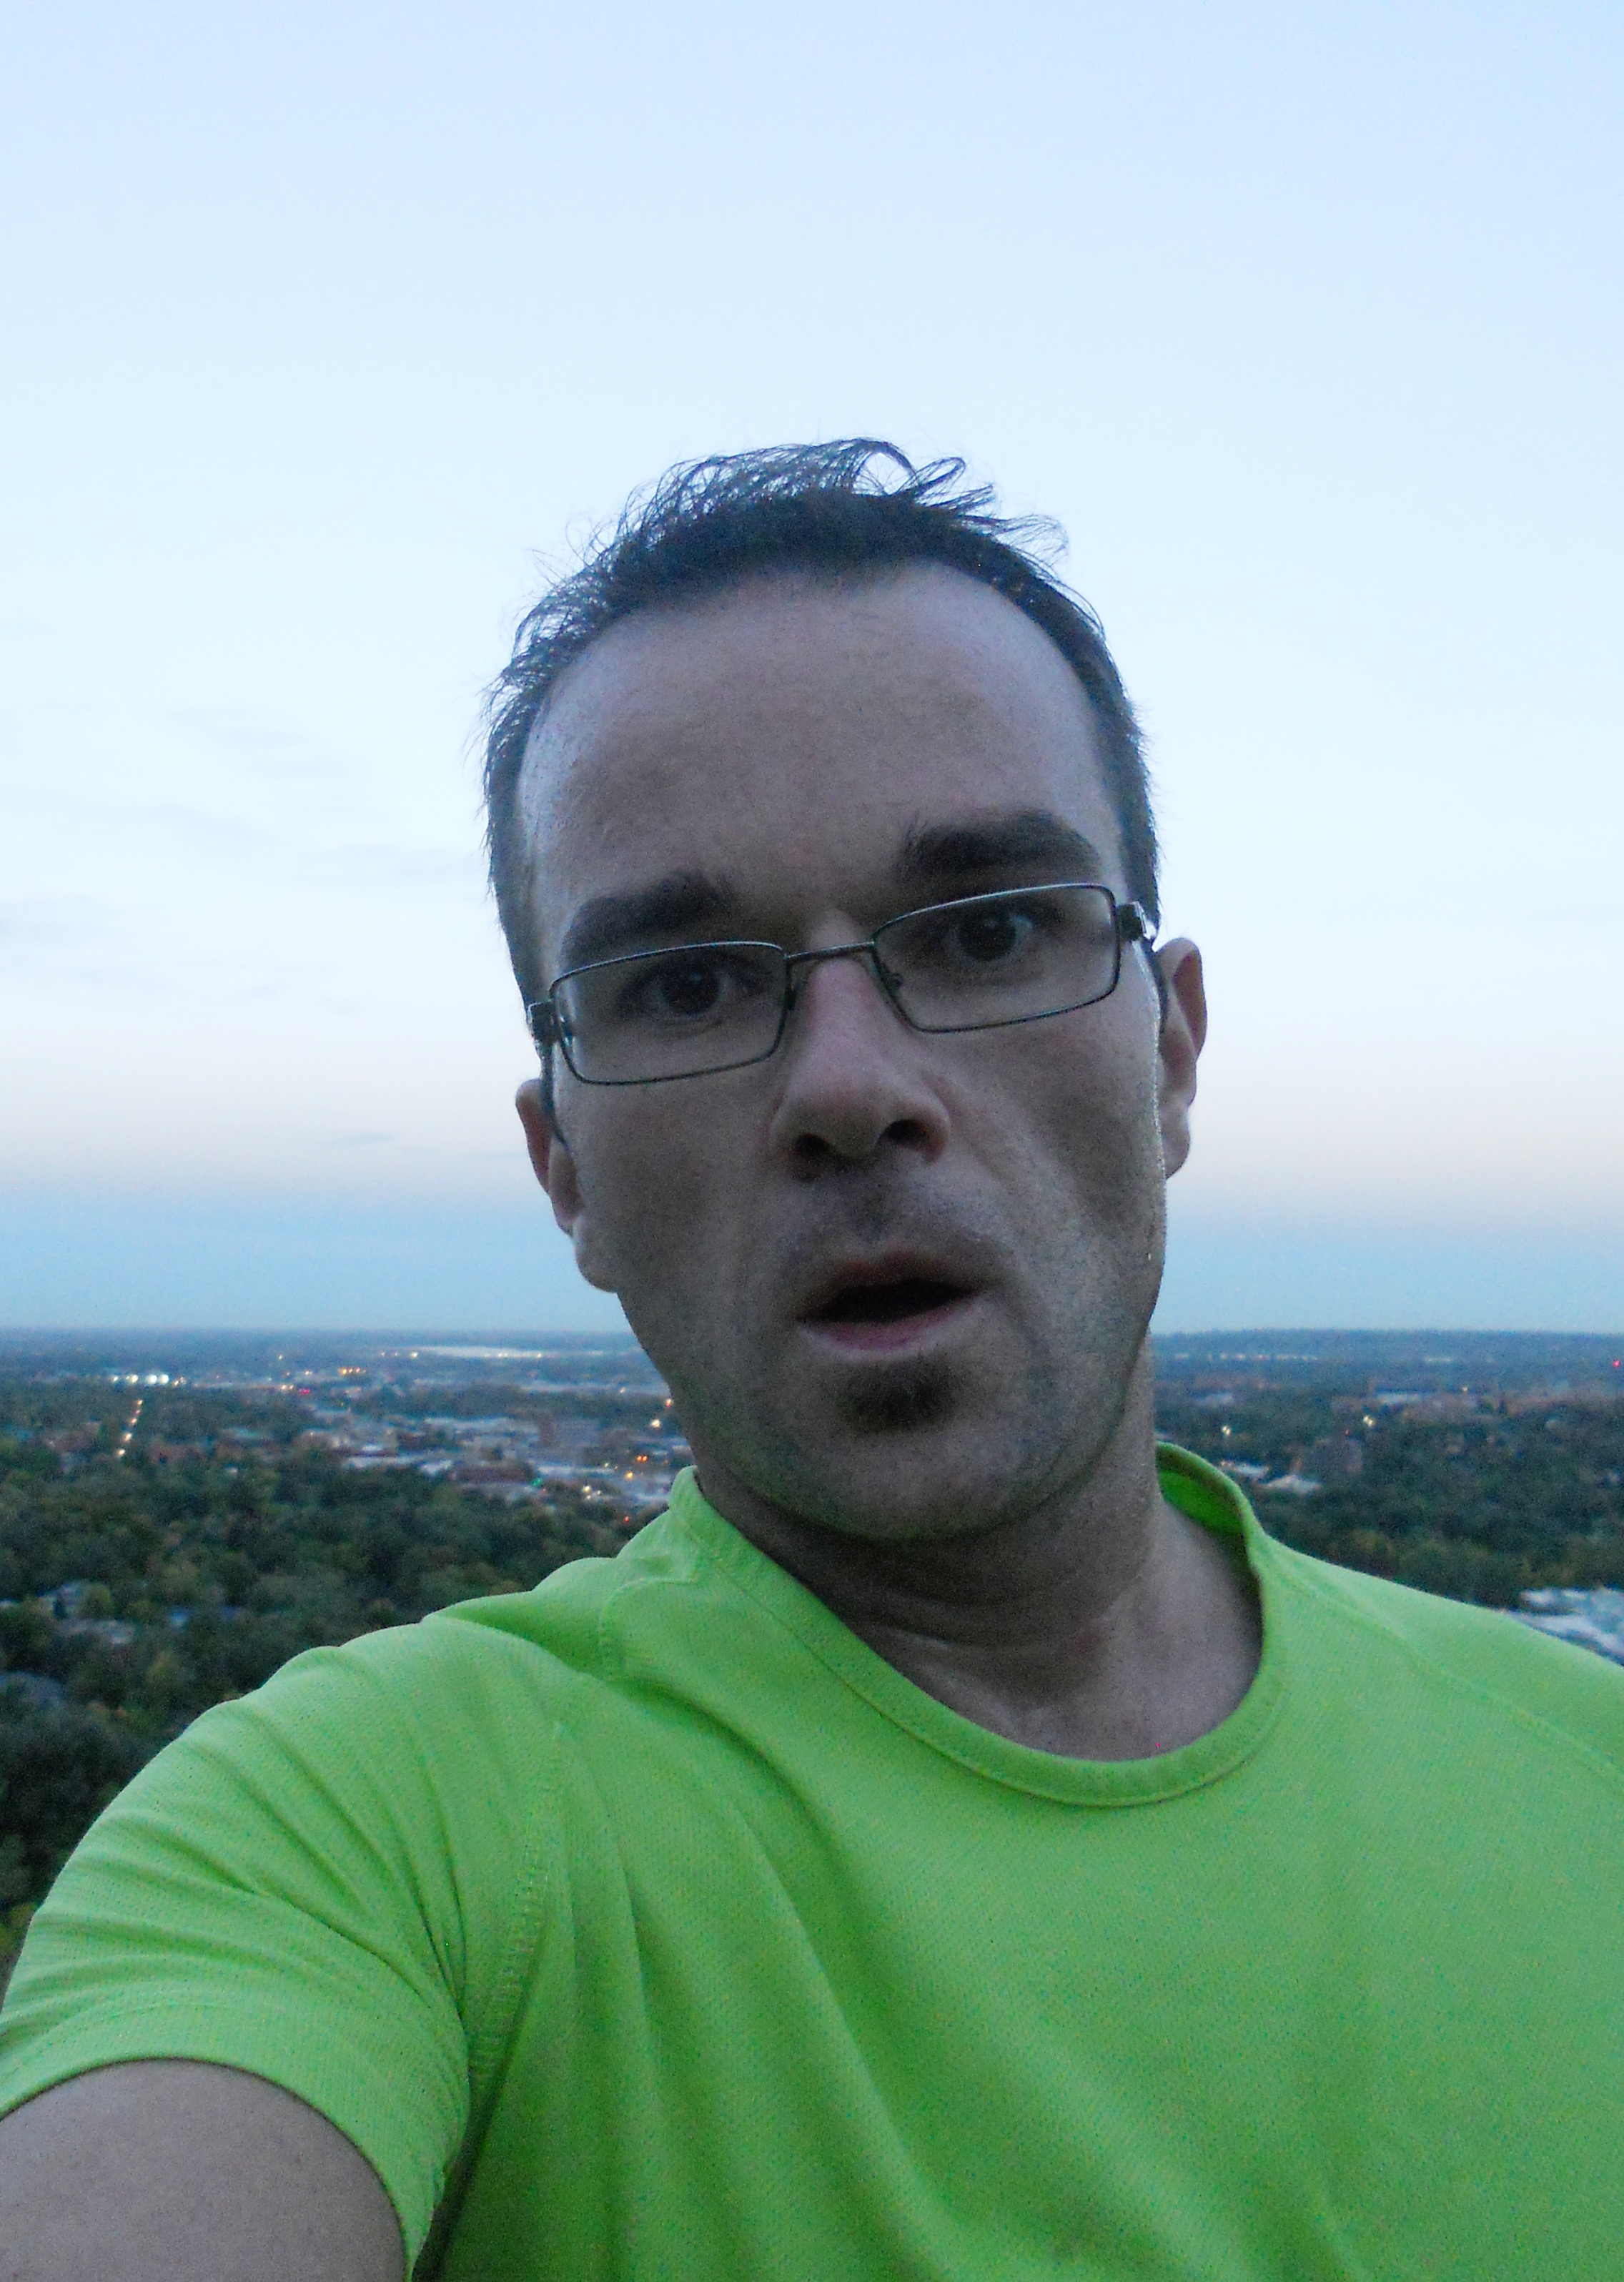
\includegraphics[width=.15\textwidth]{ctroupin.jpg} & Charles && 
\includegraphics[width=.15\textwidth]{gaelle.jpg} & Gaëlle 


\end{tabular}



\end{frame}


\end{document}




%--------------------------------------------------------------------------------------------------------

\begin{frame}[t]
\frametitle{Nice or ugly?}

\begin{overlayarea}{\textwidth}{6.5cm}
\begin{figure}
\centering
\includegraphics<1>[width=.8\paperwidth]{medsea_data}
\includegraphics<2>[width=.8\paperwidth]{results2smooth}
\includegraphics<3>[width=.8\paperwidth]{results2noisy}
\includegraphics<4>[width=.8\paperwidth]{results_slightlybetter}
\includegraphics<5>[width=.8\paperwidth]{results_ok}
\end{figure}
\end{overlayarea}

\onslide*<1>{Salinity in the Mediterranean Sea}
\onslide*<2>{Too smooth!}
\onslide*<3>{Too noisy!}
\onslide*<4>{Slightly better\ldots}
\onslide*<5>{OK, looks nice!}

\end{frame}

%--------------------------------------------------------------------------------------------------------





% -------------------------------------------------------------------------------------------------------------------------------------
\end{document}
